\documentclass[1p]{elsarticle_modified}
%\bibliographystyle{elsarticle-num}

%\usepackage[colorlinks]{hyperref}
%\usepackage{abbrmath_seonhwa} %\Abb, \Ascr, \Acal ,\Abf, \Afrak
\usepackage{amsfonts}
\usepackage{amssymb}
\usepackage{amsmath}
\usepackage{amsthm}
\usepackage{scalefnt}
\usepackage{amsbsy}
\usepackage{kotex}
\usepackage{caption}
\usepackage{subfig}
\usepackage{color}
\usepackage{graphicx}
\usepackage{xcolor} %% white, black, red, green, blue, cyan, magenta, yellow
\usepackage{float}
\usepackage{setspace}
\usepackage{hyperref}

\usepackage{tikz}
\usetikzlibrary{arrows}

\usepackage{multirow}
\usepackage{array} % fixed length table
\usepackage{hhline}

%%%%%%%%%%%%%%%%%%%%%
\makeatletter
\renewcommand*\env@matrix[1][\arraystretch]{%
	\edef\arraystretch{#1}%
	\hskip -\arraycolsep
	\let\@ifnextchar\new@ifnextchar
	\array{*\c@MaxMatrixCols c}}
\makeatother %https://tex.stackexchange.com/questions/14071/how-can-i-increase-the-line-spacing-in-a-matrix
%%%%%%%%%%%%%%%

\usepackage[normalem]{ulem}

\newcommand{\msout}[1]{\ifmmode\text{\sout{\ensuremath{#1}}}\else\sout{#1}\fi}
%SOURCE: \msout is \stkout macro in https://tex.stackexchange.com/questions/20609/strikeout-in-math-mode

\newcommand{\cancel}[1]{
	\ifmmode
	{\color{red}\msout{#1}}
	\else
	{\color{red}\sout{#1}}
	\fi
}

\newcommand{\add}[1]{
	{\color{blue}\uwave{#1}}
}

\newcommand{\replace}[2]{
	\ifmmode
	{\color{red}\msout{#1}}{\color{blue}\uwave{#2}}
	\else
	{\color{red}\sout{#1}}{\color{blue}\uwave{#2}}
	\fi
}

\newcommand{\Sol}{\mathcal{S}} %segment
\newcommand{\D}{D} %diagram
\newcommand{\A}{\mathcal{A}} %arc


%%%%%%%%%%%%%%%%%%%%%%%%%%%%%5 test

\def\sl{\operatorname{\textup{SL}}(2,\Cbb)}
\def\psl{\operatorname{\textup{PSL}}(2,\Cbb)}
\def\quan{\mkern 1mu \triangleright \mkern 1mu}

\theoremstyle{definition}
\newtheorem{thm}{Theorem}[section]
\newtheorem{prop}[thm]{Proposition}
\newtheorem{lem}[thm]{Lemma}
\newtheorem{ques}[thm]{Question}
\newtheorem{cor}[thm]{Corollary}
\newtheorem{defn}[thm]{Definition}
\newtheorem{exam}[thm]{Example}
\newtheorem{rmk}[thm]{Remark}
\newtheorem{alg}[thm]{Algorithm}

\newcommand{\I}{\sqrt{-1}}
\begin{document}

%\begin{frontmatter}
%
%\title{Boundary parabolic representations of knots up to 8 crossings}
%
%%% Group authors per affiliation:
%\author{Yunhi Cho} 
%\address{Department of Mathematics, University of Seoul, Seoul, Korea}
%\ead{yhcho@uos.ac.kr}
%
%
%\author{Seonhwa Kim} %\fnref{s_kim}}
%\address{Center for Geometry and Physics, Institute for Basic Science, Pohang, 37673, Korea}
%\ead{ryeona17@ibs.re.kr}
%
%\author{Hyuk Kim}
%\address{Department of Mathematical Sciences, Seoul National University, Seoul 08826, Korea}
%\ead{hyukkim@snu.ac.kr}
%
%\author{Seokbeom Yoon}
%\address{Department of Mathematical Sciences, Seoul National University, Seoul, 08826,  Korea}
%\ead{sbyoon15@snu.ac.kr}
%
%\begin{abstract}
%We find all boundary parabolic representation of knots up to 8 crossings.
%
%\end{abstract}
%\begin{keyword}
%    \MSC[2010] 57M25 
%\end{keyword}
%
%\end{frontmatter}

%\linenumbers
%\tableofcontents
%
\newcommand\colored[1]{\textcolor{white}{\rule[-0.35ex]{0.8em}{1.4ex}}\kern-0.8em\color{red} #1}%
%\newcommand\colored[1]{\textcolor{white}{ #1}\kern-2.17ex	\textcolor{white}{ #1}\kern-1.81ex	\textcolor{white}{ #1}\kern-2.15ex\color{red}#1	}

{\Large $\underline{11a_{212}~(K11a_{212})}$}

\setlength{\tabcolsep}{10pt}
\renewcommand{\arraystretch}{1.6}
\vspace{1cm}\begin{tabular}{m{100pt}>{\centering\arraybackslash}m{274pt}}
\multirow{5}{120pt}{
	\centering
	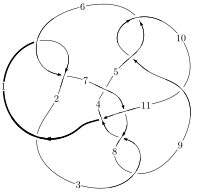
\includegraphics[width=112pt]{../../../GIT/diagram.site/Diagrams/png/461_11a_212.png}\\
\ \ \ A knot diagram\footnotemark}&
\allowdisplaybreaks
\textbf{Linearized knot diagam} \\
\cline{2-2}
 &
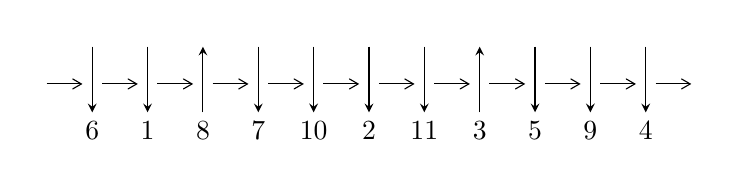
\begin{tikzpicture}[x=20pt, y=17pt]
	% nodes
	\node (C0) at (0, 0) {};
	\node (C1) at (1, 0) {};
	\node (C1U) at (1, +1) {};
	\node (C1D) at (1, -1) {6};

	\node (C2) at (2, 0) {};
	\node (C2U) at (2, +1) {};
	\node (C2D) at (2, -1) {1};

	\node (C3) at (3, 0) {};
	\node (C3U) at (3, +1) {};
	\node (C3D) at (3, -1) {8};

	\node (C4) at (4, 0) {};
	\node (C4U) at (4, +1) {};
	\node (C4D) at (4, -1) {7};

	\node (C5) at (5, 0) {};
	\node (C5U) at (5, +1) {};
	\node (C5D) at (5, -1) {10};

	\node (C6) at (6, 0) {};
	\node (C6U) at (6, +1) {};
	\node (C6D) at (6, -1) {2};

	\node (C7) at (7, 0) {};
	\node (C7U) at (7, +1) {};
	\node (C7D) at (7, -1) {11};

	\node (C8) at (8, 0) {};
	\node (C8U) at (8, +1) {};
	\node (C8D) at (8, -1) {3};

	\node (C9) at (9, 0) {};
	\node (C9U) at (9, +1) {};
	\node (C9D) at (9, -1) {5};

	\node (C10) at (10, 0) {};
	\node (C10U) at (10, +1) {};
	\node (C10D) at (10, -1) {9};

	\node (C11) at (11, 0) {};
	\node (C11U) at (11, +1) {};
	\node (C11D) at (11, -1) {4};
	\node (C12) at (12, 0) {};

	% arrows
	\draw[->,>={angle 60}]
	(C0) edge (C1) (C1) edge (C2) (C2) edge (C3) (C3) edge (C4) (C4) edge (C5) (C5) edge (C6) (C6) edge (C7) (C7) edge (C8) (C8) edge (C9) (C9) edge (C10) (C10) edge (C11) (C11) edge (C12) ;	\draw[->,>=stealth]
	(C1U) edge (C1D) (C2U) edge (C2D) (C3D) edge (C3U) (C4U) edge (C4D) (C5U) edge (C5D) (C6U) edge (C6D) (C7U) edge (C7D) (C8D) edge (C8U) (C9U) edge (C9D) (C10U) edge (C10D) (C11U) edge (C11D) ;
	\end{tikzpicture} \\
\hhline{~~} \\& 
\textbf{Solving Sequence} \\ \cline{2-2} 
 &
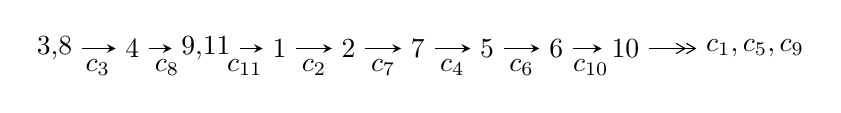
\begin{tikzpicture}[x=25pt, y=7pt]
	% node
	\node (A0) at (-1/8, 0) {3,8};
	\node (A1) at (1, 0) {4};
	\node (A2) at (33/16, 0) {9,11};
	\node (A3) at (25/8, 0) {1};
	\node (A4) at (33/8, 0) {2};
	\node (A5) at (41/8, 0) {7};
	\node (A6) at (49/8, 0) {5};
	\node (A7) at (57/8, 0) {6};
	\node (A8) at (65/8, 0) {10};
	\node (C1) at (1/2, -1) {$c_{3}$};
	\node (C2) at (3/2, -1) {$c_{8}$};
	\node (C3) at (21/8, -1) {$c_{11}$};
	\node (C4) at (29/8, -1) {$c_{2}$};
	\node (C5) at (37/8, -1) {$c_{7}$};
	\node (C6) at (45/8, -1) {$c_{4}$};
	\node (C7) at (53/8, -1) {$c_{6}$};
	\node (C8) at (61/8, -1) {$c_{10}$};
	\node (A9) at (10, 0) {$c_{1},c_{5},c_{9}$};

	% edge
	\draw[->,>=stealth]	
	(A0) edge (A1) (A1) edge (A2) (A2) edge (A3) (A3) edge (A4) (A4) edge (A5) (A5) edge (A6) (A6) edge (A7) (A7) edge (A8) ;
	\draw[->>,>={angle 60}]	
	(A8) edge (A9);
\end{tikzpicture} \\ 

\end{tabular} \\

\footnotetext{
The image of knot diagram is generated by the software ``\textbf{Draw programme}" developed by Andrew Bartholomew(\url{http://www.layer8.co.uk/maths/draw/index.htm\#Running-draw}), where we modified some parts for our purpose(\url{https://github.com/CATsTAILs/LinksPainter}).
}\phantom \\ \newline 
\centering \textbf{Ideals for irreducible components\footnotemark of $X_{\text{par}}$} 
 
\begin{align*}
I^u_{1}&=\langle 
-10169 u^{18}-100279 u^{17}+\cdots+16444 b+115784,\\
\phantom{I^u_{1}}&\phantom{= \langle  }-15886 u^{18}-173333 u^{17}+\cdots+147996 a-951450,\;u^{19}+11 u^{18}+\cdots-408 u-72\rangle \\
I^u_{2}&=\langle 
-75 u^{35}+383 u^{34}+\cdots+8 b+212,\;636 u^{35} a+43 u^{35}+\cdots+1470 a-238,\;u^{36}-5 u^{35}+\cdots-16 u+3\rangle \\
I^u_{3}&=\langle 
-2 u^7+5 u^6-11 u^5+12 u^4-11 u^3+6 u^2+b-5 u+1,\;-2 u^7+3 u^6-7 u^5+3 u^4-3 u^3- u^2+a-2 u-2,\\
\phantom{I^u_{3}}&\phantom{= \langle  }u^8-2 u^7+5 u^6-5 u^5+6 u^4-4 u^3+4 u^2- u+1\rangle \\
I^u_{4}&=\langle 
u^2 a- u^3+a u- u^2+b- u+1,\;- u^3 a-2 u^2 a+2 u^3+a^2-3 a u+2 u^2- a+3 u-1,\;u^4+u^3+2 u^2+1\rangle \\
\\
I^v_{1}&=\langle 
a,\;b-1,\;v-1\rangle \\
\end{align*}
\raggedright * 5 irreducible components of $\dim_{\mathbb{C}}=0$, with total 108 representations.\\
\footnotetext{All coefficients of polynomials are rational numbers. But the coefficients are sometimes approximated in decimal forms when there is not enough margin.}
\newpage
\renewcommand{\arraystretch}{1}
\centering \section*{I. $I^u_{1}= \langle -1.02\times10^{4} u^{18}-1.00\times10^{5} u^{17}+\cdots+1.64\times10^{4} b+1.16\times10^{5},\;-1.59\times10^{4} u^{18}-1.73\times10^{5} u^{17}+\cdots+1.48\times10^{5} a-9.51\times10^{5},\;u^{19}+11 u^{18}+\cdots-408 u-72 \rangle$}
\flushleft \textbf{(i) Arc colorings}\\
\begin{tabular}{m{7pt} m{180pt} m{7pt} m{180pt} }
\flushright $a_{3}=$&$\begin{pmatrix}1\\0\end{pmatrix}$ \\
\flushright $a_{8}=$&$\begin{pmatrix}0\\u\end{pmatrix}$ \\
\flushright $a_{4}=$&$\begin{pmatrix}1\\- u^2\end{pmatrix}$ \\
\flushright $a_{9}=$&$\begin{pmatrix}u\\u\end{pmatrix}$ \\
\flushright $a_{11}=$&$\begin{pmatrix}0.107341 u^{18}+1.17120 u^{17}+\cdots+18.8285 u+6.42889\\0.618402 u^{18}+6.09821 u^{17}+\cdots-54.0570 u-7.04111\end{pmatrix}$ \\
\flushright $a_{1}=$&$\begin{pmatrix}0.0977932 u^{18}+0.457323 u^{17}+\cdots+69.0524 u+14.1574\\-0.694661 u^{18}-7.34791 u^{17}+\cdots+195.043 u+36.7964\end{pmatrix}$ \\
\flushright $a_{2}=$&$\begin{pmatrix}-0.222793 u^{18}-2.08232 u^{17}+\cdots+5.44757 u-0.157423\\-0.0553393 u^{18}-0.402092 u^{17}+\cdots+28.9571 u+8.20360\end{pmatrix}$ \\
\flushright $a_{7}=$&$\begin{pmatrix}-0.324472 u^{18}-2.74858 u^{17}+\cdots-8.23791 u-2.15037\\0.157869 u^{18}+2.29762 u^{17}+\cdots-175.909 u-35.7215\end{pmatrix}$ \\
\flushright $a_{5}=$&$\begin{pmatrix}-0.480381 u^{18}-5.30821 u^{17}+\cdots+103.723 u+14.5621\\-0.150389 u^{18}-1.42623 u^{17}+\cdots-84.6227 u-22.7665\end{pmatrix}$ \\
\flushright $a_{6}=$&$\begin{pmatrix}-0.901210 u^{18}-9.04017 u^{17}+\cdots+115.314 u+16.7261\\-0.348699 u^{18}-2.61384 u^{17}+\cdots-168.918 u-39.7808\end{pmatrix}$ \\
\flushright $a_{10}=$&$\begin{pmatrix}0.400700 u^{18}+4.88295 u^{17}+\cdots-227.797 u-43.5867\\0.911761 u^{18}+9.80996 u^{17}+\cdots-300.682 u-57.0567\end{pmatrix}$\\ \flushright $a_{10}=$&$\begin{pmatrix}0.400700 u^{18}+4.88295 u^{17}+\cdots-227.797 u-43.5867\\0.911761 u^{18}+9.80996 u^{17}+\cdots-300.682 u-57.0567\end{pmatrix}$\\&\end{tabular}
\flushleft \textbf{(ii) Obstruction class $= -1$}\\~\\
\flushleft \textbf{(iii) Cusp Shapes $= -\frac{4653}{4111} u^{18}-\frac{45527}{4111} u^{17}+\cdots+\frac{398988}{4111} u+\frac{53874}{4111}$}\\~\\
\newpage\renewcommand{\arraystretch}{1}
\flushleft \textbf{(iv) u-Polynomials at the component}\newline \\
\begin{tabular}{m{50pt}|m{274pt}}
Crossings & \hspace{64pt}u-Polynomials at each crossing \\
\hline $$\begin{aligned}c_{1},c_{5},c_{6}\\c_{9}\end{aligned}$$&$\begin{aligned}
&u^{19}+u^{18}+\cdots+2 u+1
\end{aligned}$\\
\hline $$\begin{aligned}c_{2},c_{10}\end{aligned}$$&$\begin{aligned}
&u^{19}+9 u^{18}+\cdots-2 u+1
\end{aligned}$\\
\hline $$\begin{aligned}c_{3},c_{8}\end{aligned}$$&$\begin{aligned}
&u^{19}-11 u^{18}+\cdots-408 u+72
\end{aligned}$\\
\hline $$\begin{aligned}c_{4}\end{aligned}$$&$\begin{aligned}
&u^{19}-17 u^{18}+\cdots-1920 u+256
\end{aligned}$\\
\hline $$\begin{aligned}c_{7},c_{11}\end{aligned}$$&$\begin{aligned}
&u^{19}-2 u^{18}+\cdots+u+1
\end{aligned}$\\
\hline
\end{tabular}\\~\\
\newpage\renewcommand{\arraystretch}{1}
\flushleft \textbf{(v) Riley Polynomials at the component}\newline \\
\begin{tabular}{m{50pt}|m{274pt}}
Crossings & \hspace{64pt}Riley Polynomials at each crossing \\
\hline $$\begin{aligned}c_{1},c_{5},c_{6}\\c_{9}\end{aligned}$$&$\begin{aligned}
&y^{19}-9 y^{18}+\cdots-2 y-1
\end{aligned}$\\
\hline $$\begin{aligned}c_{2},c_{10}\end{aligned}$$&$\begin{aligned}
&y^{19}+7 y^{18}+\cdots+26 y-1
\end{aligned}$\\
\hline $$\begin{aligned}c_{3},c_{8}\end{aligned}$$&$\begin{aligned}
&y^{19}+11 y^{18}+\cdots+2016 y-5184
\end{aligned}$\\
\hline $$\begin{aligned}c_{4}\end{aligned}$$&$\begin{aligned}
&y^{19}- y^{18}+\cdots+245760 y-65536
\end{aligned}$\\
\hline $$\begin{aligned}c_{7},c_{11}\end{aligned}$$&$\begin{aligned}
&y^{19}-6 y^{18}+\cdots+27 y-1
\end{aligned}$\\
\hline
\end{tabular}\\~\\
\newpage\flushleft \textbf{(vi) Complex Volumes and Cusp Shapes}
$$\begin{array}{c|c|c}  
\text{Solutions to }I^u_{1}& \I (\text{vol} + \sqrt{-1}CS) & \text{Cusp shape}\\
 \hline 
\begin{aligned}
u &= -0.358353 + 0.924986 I \\
a &= -0.311412 + 0.717346 I \\
b &= -0.150073 + 0.860307 I\end{aligned}
 & -0.58834 - 1.54269 I & -4.69839 + 4.51597 I \\ \hline\begin{aligned}
u &= -0.358353 - 0.924986 I \\
a &= -0.311412 - 0.717346 I \\
b &= -0.150073 - 0.860307 I\end{aligned}
 & -0.58834 + 1.54269 I & -4.69839 - 4.51597 I \\ \hline\begin{aligned}
u &= -0.966676 + 0.332222 I \\
a &= -0.818238 + 0.627994 I \\
b &= -0.311396 - 0.164177 I\end{aligned}
 & \phantom{-}4.64927 + 0.26455 I & -1.71990 + 1.02803 I \\ \hline\begin{aligned}
u &= -0.966676 - 0.332222 I \\
a &= -0.818238 - 0.627994 I \\
b &= -0.311396 + 0.164177 I\end{aligned}
 & \phantom{-}4.64927 - 0.26455 I & -1.71990 - 1.02803 I \\ \hline\begin{aligned}
u &= -0.161360 + 1.222540 I \\
a &= \phantom{-}0.464053 - 1.047230 I \\
b &= -0.11073 - 2.09115 I\end{aligned}
 & -8.96802 - 0.88990 I & -16.2208 + 0.4171 I \\ \hline\begin{aligned}
u &= -0.161360 - 1.222540 I \\
a &= \phantom{-}0.464053 + 1.047230 I \\
b &= -0.11073 + 2.09115 I\end{aligned}
 & -8.96802 + 0.88990 I & -16.2208 - 0.4171 I \\ \hline\begin{aligned}
u &= -1.289970 + 0.199680 I \\
a &= \phantom{-}0.686320 - 0.541724 I \\
b &= -0.058453 + 0.397559 I\end{aligned}
 & \phantom{-}1.64114 + 11.01570 I & -7.29016 - 9.56628 I \\ \hline\begin{aligned}
u &= -1.289970 - 0.199680 I \\
a &= \phantom{-}0.686320 + 0.541724 I \\
b &= -0.058453 - 0.397559 I\end{aligned}
 & \phantom{-}1.64114 - 11.01570 I & -7.29016 + 9.56628 I \\ \hline\begin{aligned}
u &= -0.957767 + 0.906773 I \\
a &= \phantom{-}0.311369 + 0.803824 I \\
b &= -0.398706 + 0.951941 I\end{aligned}
 & -2.39512 + 0.38448 I & -10.41076 - 2.93354 I \\ \hline\begin{aligned}
u &= -0.957767 - 0.906773 I \\
a &= \phantom{-}0.311369 - 0.803824 I \\
b &= -0.398706 - 0.951941 I\end{aligned}
 & -2.39512 - 0.38448 I & -10.41076 + 2.93354 I\\
 \hline 
 \end{array}$$\newpage$$\begin{array}{c|c|c}  
\text{Solutions to }I^u_{1}& \I (\text{vol} + \sqrt{-1}CS) & \text{Cusp shape}\\
 \hline 
\begin{aligned}
u &= -0.580441 + 1.193400 I \\
a &= -0.361294 + 1.095690 I \\
b &= -0.81291 + 1.75794 I\end{aligned}
 & \phantom{-}1.92326 - 5.83662 I & -4.80851 + 2.86417 I \\ \hline\begin{aligned}
u &= -0.580441 - 1.193400 I \\
a &= -0.361294 - 1.095690 I \\
b &= -0.81291 - 1.75794 I\end{aligned}
 & \phantom{-}1.92326 + 5.83662 I & -4.80851 - 2.86417 I \\ \hline\begin{aligned}
u &= \phantom{-}0.601065\phantom{ +0.000000I} \\
a &= -0.393184\phantom{ +0.000000I} \\
b &= \phantom{-}0.378379\phantom{ +0.000000I}\end{aligned}
 & -1.08922\phantom{ +0.000000I} & -8.82220\phantom{ +0.000000I} \\ \hline\begin{aligned}
u &= -0.65100 + 1.34345 I \\
a &= \phantom{-}0.271854 - 1.066410 I \\
b &= \phantom{-}0.98510 - 2.05670 I\end{aligned}
 & -2.0202 - 17.7092 I & -9.44410 + 10.28902 I \\ \hline\begin{aligned}
u &= -0.65100 - 1.34345 I \\
a &= \phantom{-}0.271854 + 1.066410 I \\
b &= \phantom{-}0.98510 + 2.05670 I\end{aligned}
 & -2.0202 + 17.7092 I & -9.44410 - 10.28902 I \\ \hline\begin{aligned}
u &= -0.88646 + 1.29579 I \\
a &= -0.280005 - 0.575557 I \\
b &= \phantom{-}0.078111 - 1.304770 I\end{aligned}
 & -3.47013 - 7.94178 I & -12.2006 + 9.0681 I \\ \hline\begin{aligned}
u &= -0.88646 - 1.29579 I \\
a &= -0.280005 + 0.575557 I \\
b &= \phantom{-}0.078111 + 1.304770 I\end{aligned}
 & -3.47013 + 7.94178 I & -12.2006 - 9.0681 I \\ \hline\begin{aligned}
u &= \phantom{-}0.05150 + 1.63379 I \\
a &= \phantom{-}0.067278 - 0.325219 I \\
b &= -0.410127 - 0.971726 I\end{aligned}
 & -5.85414 + 4.86122 I & -16.7957 - 3.2884 I \\ \hline\begin{aligned}
u &= \phantom{-}0.05150 - 1.63379 I \\
a &= \phantom{-}0.067278 + 0.325219 I \\
b &= -0.410127 + 0.971726 I\end{aligned}
 & -5.85414 - 4.86122 I & -16.7957 + 3.2884 I\\
 \hline 
 \end{array}$$\newpage\newpage\renewcommand{\arraystretch}{1}
\centering \section*{II. $I^u_{2}= \langle -75 u^{35}+383 u^{34}+\cdots+8 b+212,\;636 u^{35} a+43 u^{35}+\cdots+1470 a-238,\;u^{36}-5 u^{35}+\cdots-16 u+3 \rangle$}
\flushleft \textbf{(i) Arc colorings}\\
\begin{tabular}{m{7pt} m{180pt} m{7pt} m{180pt} }
\flushright $a_{3}=$&$\begin{pmatrix}1\\0\end{pmatrix}$ \\
\flushright $a_{8}=$&$\begin{pmatrix}0\\u\end{pmatrix}$ \\
\flushright $a_{4}=$&$\begin{pmatrix}1\\- u^2\end{pmatrix}$ \\
\flushright $a_{9}=$&$\begin{pmatrix}u\\u\end{pmatrix}$ \\
\flushright $a_{11}=$&$\begin{pmatrix}a\\9.37500 u^{35}-47.8750 u^{34}+\cdots+161.750 u-26.5000\end{pmatrix}$ \\
\flushright $a_{1}=$&$\begin{pmatrix}-\frac{75}{8} u^{35}+\frac{383}{8} u^{34}+\cdots+a+\frac{53}{2}\\\frac{9}{4} u^{35}-\frac{125}{8} u^{34}+\cdots+\frac{941}{8} u-\frac{47}{2}\end{pmatrix}$ \\
\flushright $a_{2}=$&$\begin{pmatrix}-3.37500 a u^{35}+1.54167 u^{35}+\cdots+21.3750 a-3.66667\\-0.250000 a u^{35}-4.75000 u^{35}+\cdots+16.5000 a+13.5000\end{pmatrix}$ \\
\flushright $a_{7}=$&$\begin{pmatrix}-9.37500 a u^{35}-3.66667 u^{35}+\cdots+26.5000 a+1.79167\\-\frac{57}{8} u^{35} a-\frac{47}{8} u^{35}+\cdots+3 a-\frac{7}{4}\end{pmatrix}$ \\
\flushright $a_{5}=$&$\begin{pmatrix}-4.87500 a u^{35}+12.2917 u^{35}+\cdots+26.7500 a-25.7917\\-7.37500 a u^{35}+13.5000 u^{35}+\cdots+17.6250 a-23.3750\end{pmatrix}$ \\
\flushright $a_{6}=$&$\begin{pmatrix}5.87500 a u^{35}+13.7083 u^{35}+\cdots+2.75000 a-6.33333\\1.62500 a u^{35}+4.87500 u^{35}+\cdots+12.7500 a-26.7500\end{pmatrix}$ \\
\flushright $a_{10}=$&$\begin{pmatrix}-\frac{57}{8} u^{35}+\frac{129}{4} u^{34}+\cdots+a+3\\\frac{9}{4} u^{35}-\frac{125}{8} u^{34}+\cdots+\frac{941}{8} u-\frac{47}{2}\end{pmatrix}$\\ \flushright $a_{10}=$&$\begin{pmatrix}-\frac{57}{8} u^{35}+\frac{129}{4} u^{34}+\cdots+a+3\\\frac{9}{4} u^{35}-\frac{125}{8} u^{34}+\cdots+\frac{941}{8} u-\frac{47}{2}\end{pmatrix}$\\&\end{tabular}
\flushleft \textbf{(ii) Obstruction class $= -1$}\\~\\
\flushleft \textbf{(iii) Cusp Shapes $= \frac{47}{2} u^{35}-\frac{211}{2} u^{34}+\cdots+73 u+\frac{3}{2}$}\\~\\
\newpage\renewcommand{\arraystretch}{1}
\flushleft \textbf{(iv) u-Polynomials at the component}\newline \\
\begin{tabular}{m{50pt}|m{274pt}}
Crossings & \hspace{64pt}u-Polynomials at each crossing \\
\hline $$\begin{aligned}c_{1},c_{5},c_{6}\\c_{9}\end{aligned}$$&$\begin{aligned}
&u^{72}- u^{71}+\cdots-26 u+43
\end{aligned}$\\
\hline $$\begin{aligned}c_{2},c_{10}\end{aligned}$$&$\begin{aligned}
&u^{72}+29 u^{71}+\cdots+25272 u+1849
\end{aligned}$\\
\hline $$\begin{aligned}c_{3},c_{8}\end{aligned}$$&$\begin{aligned}
&(u^{36}+5 u^{35}+\cdots+16 u+3)^{2}
\end{aligned}$\\
\hline $$\begin{aligned}c_{4}\end{aligned}$$&$\begin{aligned}
&(u^{36}+7 u^{35}+\cdots+10 u+1)^{2}
\end{aligned}$\\
\hline $$\begin{aligned}c_{7},c_{11}\end{aligned}$$&$\begin{aligned}
&u^{72}-2 u^{71}+\cdots-22 u+1
\end{aligned}$\\
\hline
\end{tabular}\\~\\
\newpage\renewcommand{\arraystretch}{1}
\flushleft \textbf{(v) Riley Polynomials at the component}\newline \\
\begin{tabular}{m{50pt}|m{274pt}}
Crossings & \hspace{64pt}Riley Polynomials at each crossing \\
\hline $$\begin{aligned}c_{1},c_{5},c_{6}\\c_{9}\end{aligned}$$&$\begin{aligned}
&y^{72}-29 y^{71}+\cdots-25272 y+1849
\end{aligned}$\\
\hline $$\begin{aligned}c_{2},c_{10}\end{aligned}$$&$\begin{aligned}
&y^{72}+31 y^{71}+\cdots-7699036 y+3418801
\end{aligned}$\\
\hline $$\begin{aligned}c_{3},c_{8}\end{aligned}$$&$\begin{aligned}
&(y^{36}+23 y^{35}+\cdots+140 y+9)^{2}
\end{aligned}$\\
\hline $$\begin{aligned}c_{4}\end{aligned}$$&$\begin{aligned}
&(y^{36}+7 y^{35}+\cdots-4 y+1)^{2}
\end{aligned}$\\
\hline $$\begin{aligned}c_{7},c_{11}\end{aligned}$$&$\begin{aligned}
&y^{72}-4 y^{71}+\cdots-18 y+1
\end{aligned}$\\
\hline
\end{tabular}\\~\\
\newpage\flushleft \textbf{(vi) Complex Volumes and Cusp Shapes}
$$\begin{array}{c|c|c}  
\text{Solutions to }I^u_{2}& \I (\text{vol} + \sqrt{-1}CS) & \text{Cusp shape}\\
 \hline 
\begin{aligned}
u &= \phantom{-}0.323607 + 0.937654 I \\
a &= -0.175351 - 0.450939 I \\
b &= -1.42855 - 2.11019 I\end{aligned}
 & -0.65303 + 8.38929 I & -8.7813 - 13.2523 I \\ \hline\begin{aligned}
u &= \phantom{-}0.323607 + 0.937654 I \\
a &= \phantom{-}2.11473 - 0.35700 I \\
b &= \phantom{-}1.05507 - 1.24949 I\end{aligned}
 & -0.65303 + 8.38929 I & -8.7813 - 13.2523 I \\ \hline\begin{aligned}
u &= \phantom{-}0.323607 - 0.937654 I \\
a &= -0.175351 + 0.450939 I \\
b &= -1.42855 + 2.11019 I\end{aligned}
 & -0.65303 - 8.38929 I & -8.7813 + 13.2523 I \\ \hline\begin{aligned}
u &= \phantom{-}0.323607 - 0.937654 I \\
a &= \phantom{-}2.11473 + 0.35700 I \\
b &= \phantom{-}1.05507 + 1.24949 I\end{aligned}
 & -0.65303 - 8.38929 I & -8.7813 + 13.2523 I \\ \hline\begin{aligned}
u &= -0.407223 + 0.893066 I \\
a &= -0.791967 + 0.557123 I \\
b &= \phantom{-}0.506201 + 0.724691 I\end{aligned}
 & \phantom{-}1.70318 - 0.95050 I & -2.58255 + 0.79026 I \\ \hline\begin{aligned}
u &= -0.407223 + 0.893066 I \\
a &= -0.28278 + 1.70972 I \\
b &= -1.24717 + 1.80857 I\end{aligned}
 & \phantom{-}1.70318 - 0.95050 I & -2.58255 + 0.79026 I \\ \hline\begin{aligned}
u &= -0.407223 - 0.893066 I \\
a &= -0.791967 - 0.557123 I \\
b &= \phantom{-}0.506201 - 0.724691 I\end{aligned}
 & \phantom{-}1.70318 + 0.95050 I & -2.58255 - 0.79026 I \\ \hline\begin{aligned}
u &= -0.407223 - 0.893066 I \\
a &= -0.28278 - 1.70972 I \\
b &= -1.24717 - 1.80857 I\end{aligned}
 & \phantom{-}1.70318 + 0.95050 I & -2.58255 - 0.79026 I \\ \hline\begin{aligned}
u &= \phantom{-}0.285005 + 0.986264 I \\
a &= \phantom{-}0.906188 + 0.471916 I \\
b &= -0.680137 + 0.614572 I\end{aligned}
 & \phantom{-}1.39070 + 5.45819 I & -4.75268 - 7.85090 I \\ \hline\begin{aligned}
u &= \phantom{-}0.285005 + 0.986264 I \\
a &= -0.18402 - 1.83089 I \\
b &= -0.98618 - 2.55701 I\end{aligned}
 & \phantom{-}1.39070 + 5.45819 I & -4.75268 - 7.85090 I\\
 \hline 
 \end{array}$$\newpage$$\begin{array}{c|c|c}  
\text{Solutions to }I^u_{2}& \I (\text{vol} + \sqrt{-1}CS) & \text{Cusp shape}\\
 \hline 
\begin{aligned}
u &= \phantom{-}0.285005 - 0.986264 I \\
a &= \phantom{-}0.906188 - 0.471916 I \\
b &= -0.680137 - 0.614572 I\end{aligned}
 & \phantom{-}1.39070 - 5.45819 I & -4.75268 + 7.85090 I \\ \hline\begin{aligned}
u &= \phantom{-}0.285005 - 0.986264 I \\
a &= -0.18402 + 1.83089 I \\
b &= -0.98618 + 2.55701 I\end{aligned}
 & \phantom{-}1.39070 - 5.45819 I & -4.75268 + 7.85090 I \\ \hline\begin{aligned}
u &= -0.204395 + 0.939901 I \\
a &= \phantom{-}0.159162 - 0.415191 I \\
b &= \phantom{-}1.60287 - 1.64255 I\end{aligned}
 & \phantom{-}0.14515 - 3.09361 I & -8.82386 + 5.93072 I \\ \hline\begin{aligned}
u &= -0.204395 + 0.939901 I \\
a &= \phantom{-}1.66507 + 1.03102 I \\
b &= \phantom{-}0.64754 + 1.27304 I\end{aligned}
 & \phantom{-}0.14515 - 3.09361 I & -8.82386 + 5.93072 I \\ \hline\begin{aligned}
u &= -0.204395 - 0.939901 I \\
a &= \phantom{-}0.159162 + 0.415191 I \\
b &= \phantom{-}1.60287 + 1.64255 I\end{aligned}
 & \phantom{-}0.14515 + 3.09361 I & -8.82386 - 5.93072 I \\ \hline\begin{aligned}
u &= -0.204395 - 0.939901 I \\
a &= \phantom{-}1.66507 - 1.03102 I \\
b &= \phantom{-}0.64754 - 1.27304 I\end{aligned}
 & \phantom{-}0.14515 + 3.09361 I & -8.82386 - 5.93072 I \\ \hline\begin{aligned}
u &= -0.988537 + 0.351198 I \\
a &= \phantom{-}0.225935 + 0.946460 I \\
b &= -0.0017989 - 0.1085760 I\end{aligned}
 & -1.77149 - 4.10144 I & -9.97996 + 6.24934 I \\ \hline\begin{aligned}
u &= -0.988537 + 0.351198 I \\
a &= \phantom{-}0.588772 + 0.758163 I \\
b &= -0.473418 + 0.617705 I\end{aligned}
 & -1.77149 - 4.10144 I & -9.97996 + 6.24934 I \\ \hline\begin{aligned}
u &= -0.988537 - 0.351198 I \\
a &= \phantom{-}0.225935 - 0.946460 I \\
b &= -0.0017989 + 0.1085760 I\end{aligned}
 & -1.77149 + 4.10144 I & -9.97996 - 6.24934 I \\ \hline\begin{aligned}
u &= -0.988537 - 0.351198 I \\
a &= \phantom{-}0.588772 - 0.758163 I \\
b &= -0.473418 - 0.617705 I\end{aligned}
 & -1.77149 + 4.10144 I & -9.97996 - 6.24934 I\\
 \hline 
 \end{array}$$\newpage$$\begin{array}{c|c|c}  
\text{Solutions to }I^u_{2}& \I (\text{vol} + \sqrt{-1}CS) & \text{Cusp shape}\\
 \hline 
\begin{aligned}
u &= \phantom{-}1.080650 + 0.243992 I \\
a &= -0.856190 - 0.655908 I \\
b &= -0.047350 + 0.413085 I\end{aligned}
 & \phantom{-}3.39022 - 5.68113 I & -3.92911 + 4.67272 I \\ \hline\begin{aligned}
u &= \phantom{-}1.080650 + 0.243992 I \\
a &= \phantom{-}0.724773 + 0.544582 I \\
b &= \phantom{-}0.249139 - 0.068035 I\end{aligned}
 & \phantom{-}3.39022 - 5.68113 I & -3.92911 + 4.67272 I \\ \hline\begin{aligned}
u &= \phantom{-}1.080650 - 0.243992 I \\
a &= -0.856190 + 0.655908 I \\
b &= -0.047350 - 0.413085 I\end{aligned}
 & \phantom{-}3.39022 + 5.68113 I & -3.92911 - 4.67272 I \\ \hline\begin{aligned}
u &= \phantom{-}1.080650 - 0.243992 I \\
a &= \phantom{-}0.724773 - 0.544582 I \\
b &= \phantom{-}0.249139 + 0.068035 I\end{aligned}
 & \phantom{-}3.39022 + 5.68113 I & -3.92911 - 4.67272 I \\ \hline\begin{aligned}
u &= -0.118764 + 0.883260 I \\
a &= \phantom{-}1.240850 + 0.207363 I \\
b &= -0.794679 + 0.293981 I\end{aligned}
 & \phantom{-}0.57130 + 1.50593 I & -8.88680 + 0.90138 I \\ \hline\begin{aligned}
u &= -0.118764 + 0.883260 I \\
a &= -0.11523 - 1.91114 I \\
b &= \phantom{-}0.64321 - 2.55956 I\end{aligned}
 & \phantom{-}0.57130 + 1.50593 I & -8.88680 + 0.90138 I \\ \hline\begin{aligned}
u &= -0.118764 - 0.883260 I \\
a &= \phantom{-}1.240850 - 0.207363 I \\
b &= -0.794679 - 0.293981 I\end{aligned}
 & \phantom{-}0.57130 - 1.50593 I & -8.88680 - 0.90138 I \\ \hline\begin{aligned}
u &= -0.118764 - 0.883260 I \\
a &= -0.11523 + 1.91114 I \\
b &= \phantom{-}0.64321 + 2.55956 I\end{aligned}
 & \phantom{-}0.57130 - 1.50593 I & -8.88680 - 0.90138 I \\ \hline\begin{aligned}
u &= \phantom{-}0.375701 + 1.185220 I \\
a &= -0.185369 - 0.878085 I \\
b &= \phantom{-}0.06699 - 1.99722 I\end{aligned}
 & -4.64275 + 3.93521 I & -11.18615 - 4.33934 I \\ \hline\begin{aligned}
u &= \phantom{-}0.375701 + 1.185220 I \\
a &= \phantom{-}0.543890 + 1.086350 I \\
b &= \phantom{-}0.68365 + 1.43792 I\end{aligned}
 & -4.64275 + 3.93521 I & -11.18615 - 4.33934 I\\
 \hline 
 \end{array}$$\newpage$$\begin{array}{c|c|c}  
\text{Solutions to }I^u_{2}& \I (\text{vol} + \sqrt{-1}CS) & \text{Cusp shape}\\
 \hline 
\begin{aligned}
u &= \phantom{-}0.375701 - 1.185220 I \\
a &= -0.185369 + 0.878085 I \\
b &= \phantom{-}0.06699 + 1.99722 I\end{aligned}
 & -4.64275 - 3.93521 I & -11.18615 + 4.33934 I \\ \hline\begin{aligned}
u &= \phantom{-}0.375701 - 1.185220 I \\
a &= \phantom{-}0.543890 - 1.086350 I \\
b &= \phantom{-}0.68365 - 1.43792 I\end{aligned}
 & -4.64275 - 3.93521 I & -11.18615 + 4.33934 I \\ \hline\begin{aligned}
u &= \phantom{-}0.366522 + 0.661253 I \\
a &= -1.43742 - 0.22873 I \\
b &= \phantom{-}0.789147 + 0.111369 I\end{aligned}
 & \phantom{-}0.15412 - 5.32337 I & -7.89175 + 4.81078 I \\ \hline\begin{aligned}
u &= \phantom{-}0.366522 + 0.661253 I \\
a &= -0.25927 + 1.87585 I \\
b &= \phantom{-}1.20633 + 1.72823 I\end{aligned}
 & \phantom{-}0.15412 - 5.32337 I & -7.89175 + 4.81078 I \\ \hline\begin{aligned}
u &= \phantom{-}0.366522 - 0.661253 I \\
a &= -1.43742 + 0.22873 I \\
b &= \phantom{-}0.789147 - 0.111369 I\end{aligned}
 & \phantom{-}0.15412 + 5.32337 I & -7.89175 - 4.81078 I \\ \hline\begin{aligned}
u &= \phantom{-}0.366522 - 0.661253 I \\
a &= -0.25927 - 1.87585 I \\
b &= \phantom{-}1.20633 - 1.72823 I\end{aligned}
 & \phantom{-}0.15412 + 5.32337 I & -7.89175 - 4.81078 I \\ \hline\begin{aligned}
u &= \phantom{-}0.733621 + 0.056495 I \\
a &= -0.712576 + 0.589887 I \\
b &= \phantom{-}0.390901 + 0.249697 I\end{aligned}
 & -1.027180 + 0.066620 I & -7.89585 - 0.16999 I \\ \hline\begin{aligned}
u &= \phantom{-}0.733621 + 0.056495 I \\
a &= \phantom{-}0.000334 - 0.690063 I \\
b &= \phantom{-}0.498708 - 0.023336 I\end{aligned}
 & -1.027180 + 0.066620 I & -7.89585 - 0.16999 I \\ \hline\begin{aligned}
u &= \phantom{-}0.733621 - 0.056495 I \\
a &= -0.712576 - 0.589887 I \\
b &= \phantom{-}0.390901 - 0.249697 I\end{aligned}
 & -1.027180 - 0.066620 I & -7.89585 + 0.16999 I \\ \hline\begin{aligned}
u &= \phantom{-}0.733621 - 0.056495 I \\
a &= \phantom{-}0.000334 + 0.690063 I \\
b &= \phantom{-}0.498708 + 0.023336 I\end{aligned}
 & -1.027180 - 0.066620 I & -7.89585 + 0.16999 I\\
 \hline 
 \end{array}$$\newpage$$\begin{array}{c|c|c}  
\text{Solutions to }I^u_{2}& \I (\text{vol} + \sqrt{-1}CS) & \text{Cusp shape}\\
 \hline 
\begin{aligned}
u &= \phantom{-}0.461229 + 1.192960 I \\
a &= \phantom{-}0.735450 + 0.704350 I \\
b &= \phantom{-}0.941882 + 0.432336 I\end{aligned}
 & -4.33727 + 4.33344 I & \phantom{-0.000000 } 0. - 7.98095 I \\ \hline\begin{aligned}
u &= \phantom{-}0.461229 + 1.192960 I \\
a &= -0.079786 - 0.637262 I \\
b &= -0.29680 - 1.88578 I\end{aligned}
 & -4.33727 + 4.33344 I & \phantom{-0.000000 } 0. - 7.98095 I \\ \hline\begin{aligned}
u &= \phantom{-}0.461229 - 1.192960 I \\
a &= \phantom{-}0.735450 - 0.704350 I \\
b &= \phantom{-}0.941882 - 0.432336 I\end{aligned}
 & -4.33727 - 4.33344 I & \phantom{-0.000000 -}0. + 7.98095 I \\ \hline\begin{aligned}
u &= \phantom{-}0.461229 - 1.192960 I \\
a &= -0.079786 + 0.637262 I \\
b &= -0.29680 + 1.88578 I\end{aligned}
 & -4.33727 - 4.33344 I & \phantom{-0.000000 -}0. + 7.98095 I \\ \hline\begin{aligned}
u &= \phantom{-}0.261513 + 1.263160 I \\
a &= \phantom{-}0.008648 + 0.711153 I \\
b &= \phantom{-}0.111760 + 1.082130 I\end{aligned}
 & -2.36014 - 1.61358 I & \phantom{-0.000000 } 0 \\ \hline\begin{aligned}
u &= \phantom{-}0.261513 + 1.263160 I \\
a &= \phantom{-}0.056995 - 0.282130 I \\
b &= \phantom{-}0.796685 - 0.665417 I\end{aligned}
 & -2.36014 - 1.61358 I & \phantom{-0.000000 } 0 \\ \hline\begin{aligned}
u &= \phantom{-}0.261513 - 1.263160 I \\
a &= \phantom{-}0.008648 - 0.711153 I \\
b &= \phantom{-}0.111760 - 1.082130 I\end{aligned}
 & -2.36014 + 1.61358 I & \phantom{-0.000000 } 0 \\ \hline\begin{aligned}
u &= \phantom{-}0.261513 - 1.263160 I \\
a &= \phantom{-}0.056995 + 0.282130 I \\
b &= \phantom{-}0.796685 + 0.665417 I\end{aligned}
 & -2.36014 + 1.61358 I & \phantom{-0.000000 } 0 \\ \hline\begin{aligned}
u &= -0.386093 + 1.315540 I \\
a &= \phantom{-}0.321924 - 0.776161 I \\
b &= -0.07289 - 2.11359 I\end{aligned}
 & -6.83745 - 8.51873 I & \phantom{-0.000000 } 0 \\ \hline\begin{aligned}
u &= -0.386093 + 1.315540 I \\
a &= \phantom{-}0.567468 - 1.208310 I \\
b &= \phantom{-}1.22818 - 2.05777 I\end{aligned}
 & -6.83745 - 8.51873 I & \phantom{-0.000000 } 0\\
 \hline 
 \end{array}$$\newpage$$\begin{array}{c|c|c}  
\text{Solutions to }I^u_{2}& \I (\text{vol} + \sqrt{-1}CS) & \text{Cusp shape}\\
 \hline 
\begin{aligned}
u &= -0.386093 - 1.315540 I \\
a &= \phantom{-}0.321924 + 0.776161 I \\
b &= -0.07289 + 2.11359 I\end{aligned}
 & -6.83745 + 8.51873 I & \phantom{-0.000000 } 0 \\ \hline\begin{aligned}
u &= -0.386093 - 1.315540 I \\
a &= \phantom{-}0.567468 + 1.208310 I \\
b &= \phantom{-}1.22818 + 2.05777 I\end{aligned}
 & -6.83745 + 8.51873 I & \phantom{-0.000000 } 0 \\ \hline\begin{aligned}
u &= \phantom{-}0.790023 + 1.128140 I \\
a &= -0.183542 + 0.797397 I \\
b &= \phantom{-}0.321793 + 1.049820 I\end{aligned}
 & -2.51334 + 3.34840 I & \phantom{-0.000000 } 0 \\ \hline\begin{aligned}
u &= \phantom{-}0.790023 + 1.128140 I \\
a &= \phantom{-}0.286168 - 0.668765 I \\
b &= \phantom{-}0.038092 - 1.366730 I\end{aligned}
 & -2.51334 + 3.34840 I & \phantom{-0.000000 } 0 \\ \hline\begin{aligned}
u &= \phantom{-}0.790023 - 1.128140 I \\
a &= -0.183542 - 0.797397 I \\
b &= \phantom{-}0.321793 - 1.049820 I\end{aligned}
 & -2.51334 - 3.34840 I & \phantom{-0.000000 } 0 \\ \hline\begin{aligned}
u &= \phantom{-}0.790023 - 1.128140 I \\
a &= \phantom{-}0.286168 + 0.668765 I \\
b &= \phantom{-}0.038092 + 1.366730 I\end{aligned}
 & -2.51334 - 3.34840 I & \phantom{-0.000000 } 0 \\ \hline\begin{aligned}
u &= -0.341744 + 0.520197 I \\
a &= -0.607007 + 0.115057 I \\
b &= -0.304801 + 1.331690 I\end{aligned}
 & \phantom{-}2.67726 - 2.50734 I & \phantom{-}0.46124 + 4.14494 I \\ \hline\begin{aligned}
u &= -0.341744 + 0.520197 I \\
a &= -2.20469 + 1.12056 I \\
b &= -0.885119 - 0.256430 I\end{aligned}
 & \phantom{-}2.67726 - 2.50734 I & \phantom{-}0.46124 + 4.14494 I \\ \hline\begin{aligned}
u &= -0.341744 - 0.520197 I \\
a &= -0.607007 - 0.115057 I \\
b &= -0.304801 - 1.331690 I\end{aligned}
 & \phantom{-}2.67726 + 2.50734 I & \phantom{-}0.46124 - 4.14494 I \\ \hline\begin{aligned}
u &= -0.341744 - 0.520197 I \\
a &= -2.20469 - 1.12056 I \\
b &= -0.885119 + 0.256430 I\end{aligned}
 & \phantom{-}2.67726 + 2.50734 I & \phantom{-}0.46124 - 4.14494 I\\
 \hline 
 \end{array}$$\newpage$$\begin{array}{c|c|c}  
\text{Solutions to }I^u_{2}& \I (\text{vol} + \sqrt{-1}CS) & \text{Cusp shape}\\
 \hline 
\begin{aligned}
u &= \phantom{-}0.598145 + 1.270670 I \\
a &= \phantom{-}0.364362 + 1.030040 I \\
b &= \phantom{-}0.72567 + 1.78948 I\end{aligned}
 & \phantom{-}0.12476 + 11.63330 I & \phantom{-0.000000 } 0 \\ \hline\begin{aligned}
u &= \phantom{-}0.598145 + 1.270670 I \\
a &= -0.282009 - 1.154280 I \\
b &= -1.01814 - 2.10114 I\end{aligned}
 & \phantom{-}0.12476 + 11.63330 I & \phantom{-0.000000 } 0 \\ \hline\begin{aligned}
u &= \phantom{-}0.598145 - 1.270670 I \\
a &= \phantom{-}0.364362 - 1.030040 I \\
b &= \phantom{-}0.72567 - 1.78948 I\end{aligned}
 & \phantom{-}0.12476 - 11.63330 I & \phantom{-0.000000 } 0 \\ \hline\begin{aligned}
u &= \phantom{-}0.598145 - 1.270670 I \\
a &= -0.282009 + 1.154280 I \\
b &= -1.01814 + 2.10114 I\end{aligned}
 & \phantom{-}0.12476 - 11.63330 I & \phantom{-0.000000 } 0 \\ \hline\begin{aligned}
u &= \phantom{-}0.255236 + 0.508176 I \\
a &= \phantom{-}0.494661 - 0.107326 I \\
b &= \phantom{-}0.75887 + 1.28212 I\end{aligned}
 & \phantom{-}2.67098 - 2.77341 I & -0.394325 + 0.708366 I \\ \hline\begin{aligned}
u &= \phantom{-}0.255236 + 0.508176 I \\
a &= -2.79447 - 0.04340 I \\
b &= -0.731661 + 0.492551 I\end{aligned}
 & \phantom{-}2.67098 - 2.77341 I & -0.394325 + 0.708366 I \\ \hline\begin{aligned}
u &= \phantom{-}0.255236 - 0.508176 I \\
a &= \phantom{-}0.494661 + 0.107326 I \\
b &= \phantom{-}0.75887 - 1.28212 I\end{aligned}
 & \phantom{-}2.67098 + 2.77341 I & -0.394325 - 0.708366 I \\ \hline\begin{aligned}
u &= \phantom{-}0.255236 - 0.508176 I \\
a &= -2.79447 + 0.04340 I \\
b &= -0.731661 - 0.492551 I\end{aligned}
 & \phantom{-}2.67098 + 2.77341 I & -0.394325 - 0.708366 I \\ \hline\begin{aligned}
u &= -0.58449 + 1.51506 I \\
a &= -0.162437 - 0.495879 I \\
b &= \phantom{-}0.227921 - 1.342130 I\end{aligned}
 & -5.13435 - 2.75063 I & \phantom{-0.000000 } 0 \\ \hline\begin{aligned}
u &= -0.58449 + 1.51506 I \\
a &= -0.024617 - 0.210269 I \\
b &= -0.521920 - 0.498154 I\end{aligned}
 & -5.13435 - 2.75063 I & \phantom{-0.000000 } 0\\
 \hline 
 \end{array}$$\newpage$$\begin{array}{c|c|c}  
\text{Solutions to }I^u_{2}& \I (\text{vol} + \sqrt{-1}CS) & \text{Cusp shape}\\
 \hline 
\begin{aligned}
u &= -0.58449 - 1.51506 I \\
a &= -0.162437 + 0.495879 I \\
b &= \phantom{-}0.227921 + 1.342130 I\end{aligned}
 & -5.13435 + 2.75063 I & \phantom{-0.000000 } 0 \\ \hline\begin{aligned}
u &= -0.58449 - 1.51506 I \\
a &= -0.024617 + 0.210269 I \\
b &= -0.521920 + 0.498154 I\end{aligned}
 & -5.13435 + 2.75063 I & \phantom{-0.000000 } 0\\
 \hline 
 \end{array}$$\newpage\newpage\renewcommand{\arraystretch}{1}
\centering \section*{III. $I^u_{3}= \langle -2 u^7+5 u^6+\cdots+b+1,\;-2 u^7+3 u^6+\cdots+a-2,\;u^8-2 u^7+\cdots- u+1 \rangle$}
\flushleft \textbf{(i) Arc colorings}\\
\begin{tabular}{m{7pt} m{180pt} m{7pt} m{180pt} }
\flushright $a_{3}=$&$\begin{pmatrix}1\\0\end{pmatrix}$ \\
\flushright $a_{8}=$&$\begin{pmatrix}0\\u\end{pmatrix}$ \\
\flushright $a_{4}=$&$\begin{pmatrix}1\\- u^2\end{pmatrix}$ \\
\flushright $a_{9}=$&$\begin{pmatrix}u\\u\end{pmatrix}$ \\
\flushright $a_{11}=$&$\begin{pmatrix}2 u^7-3 u^6+7 u^5-3 u^4+3 u^3+u^2+2 u+2\\2 u^7-5 u^6+11 u^5-12 u^4+11 u^3-6 u^2+5 u-1\end{pmatrix}$ \\
\flushright $a_{1}=$&$\begin{pmatrix}u^7+6 u^4-6 u^3+7 u^2-2 u+4\\2 u^7-4 u^6+9 u^5-8 u^4+7 u^3-3 u^2+3 u\end{pmatrix}$ \\
\flushright $a_{2}=$&$\begin{pmatrix}- u^7+3 u^6-7 u^5+10 u^4-11 u^3+10 u^2-7 u+4\\u^7-2 u^6+5 u^5-5 u^4+5 u^3-2 u^2+u+1\end{pmatrix}$ \\
\flushright $a_{7}=$&$\begin{pmatrix}- u^7+u^6-3 u^5- u^3-2 u^2-3\\- u^7+2 u^6-5 u^5+5 u^4-6 u^3+4 u^2-3 u\end{pmatrix}$ \\
\flushright $a_{5}=$&$\begin{pmatrix}2 u^7-5 u^6+11 u^5-13 u^4+12 u^3-9 u^2+6 u-1\\- u^6+2 u^5-5 u^4+5 u^3-6 u^2+3 u-2\end{pmatrix}$ \\
\flushright $a_{6}=$&$\begin{pmatrix}3 u^7-8 u^6+17 u^5-20 u^4+17 u^3-11 u^2+8 u-3\\-2 u^6+4 u^5-9 u^4+8 u^3-7 u^2+3 u-3\end{pmatrix}$ \\
\flushright $a_{10}=$&$\begin{pmatrix}2 u^7-2 u^6+5 u^5+2 u^4-2 u^3+6 u^2+4\\2 u^7-4 u^6+9 u^5-7 u^4+6 u^3- u^2+3 u+1\end{pmatrix}$\\ \flushright $a_{10}=$&$\begin{pmatrix}2 u^7-2 u^6+5 u^5+2 u^4-2 u^3+6 u^2+4\\2 u^7-4 u^6+9 u^5-7 u^4+6 u^3- u^2+3 u+1\end{pmatrix}$\\&\end{tabular}
\flushleft \textbf{(ii) Obstruction class $= 1$}\\~\\
\flushleft \textbf{(iii) Cusp Shapes $= -5 u^7+15 u^6-33 u^5+42 u^4-36 u^3+22 u^2-18 u-3$}\\~\\
\newpage\renewcommand{\arraystretch}{1}
\flushleft \textbf{(iv) u-Polynomials at the component}\newline \\
\begin{tabular}{m{50pt}|m{274pt}}
Crossings & \hspace{64pt}u-Polynomials at each crossing \\
\hline $$\begin{aligned}c_{1},c_{5}\end{aligned}$$&$\begin{aligned}
&u^8-2 u^6+3 u^4+u^3-2 u^2- u+1
\end{aligned}$\\
\hline $$\begin{aligned}c_{2},c_{10}\end{aligned}$$&$\begin{aligned}
&u^8+4 u^7+10 u^6+16 u^5+19 u^4+17 u^3+12 u^2+5 u+1
\end{aligned}$\\
\hline $$\begin{aligned}c_{3}\end{aligned}$$&$\begin{aligned}
&u^8-2 u^7+5 u^6-5 u^5+6 u^4-4 u^3+4 u^2- u+1
\end{aligned}$\\
\hline $$\begin{aligned}c_{4}\end{aligned}$$&$\begin{aligned}
&u^8-3 u^7+3 u^6- u^5- u^4+u^3+1
\end{aligned}$\\
\hline $$\begin{aligned}c_{6},c_{9}\end{aligned}$$&$\begin{aligned}
&u^8-2 u^6+3 u^4- u^3-2 u^2+u+1
\end{aligned}$\\
\hline $$\begin{aligned}c_{7},c_{11}\end{aligned}$$&$\begin{aligned}
&u^8- u^7+2 u^4- u^3- u^2+1
\end{aligned}$\\
\hline $$\begin{aligned}c_{8}\end{aligned}$$&$\begin{aligned}
&u^8+2 u^7+5 u^6+5 u^5+6 u^4+4 u^3+4 u^2+u+1
\end{aligned}$\\
\hline
\end{tabular}\\~\\
\newpage\renewcommand{\arraystretch}{1}
\flushleft \textbf{(v) Riley Polynomials at the component}\newline \\
\begin{tabular}{m{50pt}|m{274pt}}
Crossings & \hspace{64pt}Riley Polynomials at each crossing \\
\hline $$\begin{aligned}c_{1},c_{5},c_{6}\\c_{9}\end{aligned}$$&$\begin{aligned}
&y^8-4 y^7+10 y^6-16 y^5+19 y^4-17 y^3+12 y^2-5 y+1
\end{aligned}$\\
\hline $$\begin{aligned}c_{2},c_{10}\end{aligned}$$&$\begin{aligned}
&y^8+4 y^7+10 y^6+12 y^5+19 y^4+27 y^3+12 y^2- y+1
\end{aligned}$\\
\hline $$\begin{aligned}c_{3},c_{8}\end{aligned}$$&$\begin{aligned}
&y^8+6 y^7+17 y^6+27 y^5+34 y^4+32 y^3+20 y^2+7 y+1
\end{aligned}$\\
\hline $$\begin{aligned}c_{4}\end{aligned}$$&$\begin{aligned}
&y^8-3 y^7+y^6- y^5+5 y^4+5 y^3-2 y^2+1
\end{aligned}$\\
\hline $$\begin{aligned}c_{7},c_{11}\end{aligned}$$&$\begin{aligned}
&y^8- y^7+4 y^6-4 y^5+6 y^4-5 y^3+5 y^2-2 y+1
\end{aligned}$\\
\hline
\end{tabular}\\~\\
\newpage\flushleft \textbf{(vi) Complex Volumes and Cusp Shapes}
$$\begin{array}{c|c|c}  
\text{Solutions to }I^u_{3}& \I (\text{vol} + \sqrt{-1}CS) & \text{Cusp shape}\\
 \hline 
\begin{aligned}
u &= \phantom{-}0.792109 + 0.738037 I \\
a &= -0.382665 + 0.800987 I \\
b &= \phantom{-}0.073913 + 0.733193 I\end{aligned}
 & -2.49555 + 0.86293 I & -13.14261 - 3.03469 I \\ \hline\begin{aligned}
u &= \phantom{-}0.792109 - 0.738037 I \\
a &= -0.382665 - 0.800987 I \\
b &= \phantom{-}0.073913 - 0.733193 I\end{aligned}
 & -2.49555 - 0.86293 I & -13.14261 + 3.03469 I \\ \hline\begin{aligned}
u &= -0.289722 + 0.810357 I \\
a &= -1.207080 - 0.334530 I \\
b &= \phantom{-}0.08655 - 1.63964 I\end{aligned}
 & -0.50761 - 7.31144 I & -8.44025 + 5.07969 I \\ \hline\begin{aligned}
u &= -0.289722 - 0.810357 I \\
a &= -1.207080 + 0.334530 I \\
b &= \phantom{-}0.08655 + 1.63964 I\end{aligned}
 & -0.50761 + 7.31144 I & -8.44025 - 5.07969 I \\ \hline\begin{aligned}
u &= \phantom{-}0.010381 + 0.674737 I \\
a &= \phantom{-}1.24580 + 1.30467 I \\
b &= -0.28206 + 1.43052 I\end{aligned}
 & \phantom{-}1.91736 + 3.67399 I & -5.72808 - 5.47869 I \\ \hline\begin{aligned}
u &= \phantom{-}0.010381 - 0.674737 I \\
a &= \phantom{-}1.24580 - 1.30467 I \\
b &= -0.28206 - 1.43052 I\end{aligned}
 & \phantom{-}1.91736 - 3.67399 I & -5.72808 + 5.47869 I \\ \hline\begin{aligned}
u &= \phantom{-}0.48723 + 1.51401 I \\
a &= -0.156057 - 0.473494 I \\
b &= -0.378403 - 1.209690 I\end{aligned}
 & -5.49394 + 5.83988 I & -13.6891 - 9.4941 I \\ \hline\begin{aligned}
u &= \phantom{-}0.48723 - 1.51401 I \\
a &= -0.156057 + 0.473494 I \\
b &= -0.378403 + 1.209690 I\end{aligned}
 & -5.49394 - 5.83988 I & -13.6891 + 9.4941 I\\
 \hline 
 \end{array}$$\newpage\newpage\renewcommand{\arraystretch}{1}
\centering \section*{IV. $I^u_{4}= \langle u^2 a- u^3+a u- u^2+b- u+1,\;- u^3 a+2 u^3+\cdots- a-1,\;u^4+u^3+2 u^2+1 \rangle$}
\flushleft \textbf{(i) Arc colorings}\\
\begin{tabular}{m{7pt} m{180pt} m{7pt} m{180pt} }
\flushright $a_{3}=$&$\begin{pmatrix}1\\0\end{pmatrix}$ \\
\flushright $a_{8}=$&$\begin{pmatrix}0\\u\end{pmatrix}$ \\
\flushright $a_{4}=$&$\begin{pmatrix}1\\- u^2\end{pmatrix}$ \\
\flushright $a_{9}=$&$\begin{pmatrix}u\\u\end{pmatrix}$ \\
\flushright $a_{11}=$&$\begin{pmatrix}a\\- u^2 a+u^3- a u+u^2+u-1\end{pmatrix}$ \\
\flushright $a_{1}=$&$\begin{pmatrix}- u^3+a u- u^2+a- u+1\\- u^3 a- u^2 a- a u-1\end{pmatrix}$ \\
\flushright $a_{2}=$&$\begin{pmatrix}- u^2 a+u^3+2 u^2- a+3 u+2\\- u^3 a- u^2 a- a u+u^2- a+u+1\end{pmatrix}$ \\
\flushright $a_{7}=$&$\begin{pmatrix}u^3 a+u^2 a+a u+u^2- a+u+2\\u^3 a+u^2 a- u^3+a u- u^2- u+1\end{pmatrix}$ \\
\flushright $a_{5}=$&$\begin{pmatrix}u^3 a+u^2 a- u^3+2 a u- u^2- u+2\\- u^3+a u-2 u^2-2 u\end{pmatrix}$ \\
\flushright $a_{6}=$&$\begin{pmatrix}u^3 a+2 u^2 a+2 a u+u^2+u+1\\u^2 a- u^3+a u- u^2+a-2 u\end{pmatrix}$ \\
\flushright $a_{10}=$&$\begin{pmatrix}u^2 a- u^3- u^2+2 a- u\\- a u+a-1\end{pmatrix}$\\ \flushright $a_{10}=$&$\begin{pmatrix}u^2 a- u^3- u^2+2 a- u\\- a u+a-1\end{pmatrix}$\\&\end{tabular}
\flushleft \textbf{(ii) Obstruction class $= 1$}\\~\\
\flushleft \textbf{(iii) Cusp Shapes $= -6 u^3-6 u^2-7 u-7$}\\~\\
\newpage\renewcommand{\arraystretch}{1}
\flushleft \textbf{(iv) u-Polynomials at the component}\newline \\
\begin{tabular}{m{50pt}|m{274pt}}
Crossings & \hspace{64pt}u-Polynomials at each crossing \\
\hline $$\begin{aligned}c_{1},c_{5}\end{aligned}$$&$\begin{aligned}
&u^8-2 u^6- u^5+3 u^4+u^3-2 u^2+1
\end{aligned}$\\
\hline $$\begin{aligned}c_{2},c_{10}\end{aligned}$$&$\begin{aligned}
&u^8+4 u^7+10 u^6+17 u^5+21 u^4+17 u^3+10 u^2+4 u+1
\end{aligned}$\\
\hline $$\begin{aligned}c_{3}\end{aligned}$$&$\begin{aligned}
&(u^4+u^3+2 u^2+1)^2
\end{aligned}$\\
\hline $$\begin{aligned}c_{4}\end{aligned}$$&$\begin{aligned}
&(u^4+u^3+1)^2
\end{aligned}$\\
\hline $$\begin{aligned}c_{6},c_{9}\end{aligned}$$&$\begin{aligned}
&u^8-2 u^6+u^5+3 u^4- u^3-2 u^2+1
\end{aligned}$\\
\hline $$\begin{aligned}c_{7},c_{11}\end{aligned}$$&$\begin{aligned}
&u^8-3 u^7+3 u^6- u^5- u^4+2 u^3- u^2+1
\end{aligned}$\\
\hline $$\begin{aligned}c_{8}\end{aligned}$$&$\begin{aligned}
&(u^4- u^3+2 u^2+1)^2
\end{aligned}$\\
\hline
\end{tabular}\\~\\
\newpage\renewcommand{\arraystretch}{1}
\flushleft \textbf{(v) Riley Polynomials at the component}\newline \\
\begin{tabular}{m{50pt}|m{274pt}}
Crossings & \hspace{64pt}Riley Polynomials at each crossing \\
\hline $$\begin{aligned}c_{1},c_{5},c_{6}\\c_{9}\end{aligned}$$&$\begin{aligned}
&y^8-4 y^7+10 y^6-17 y^5+21 y^4-17 y^3+10 y^2-4 y+1
\end{aligned}$\\
\hline $$\begin{aligned}c_{2},c_{10}\end{aligned}$$&$\begin{aligned}
&y^8+4 y^7+6 y^6+15 y^5+33 y^4+15 y^3+6 y^2+4 y+1
\end{aligned}$\\
\hline $$\begin{aligned}c_{3},c_{8}\end{aligned}$$&$\begin{aligned}
&(y^4+3 y^3+6 y^2+4 y+1)^2
\end{aligned}$\\
\hline $$\begin{aligned}c_{4}\end{aligned}$$&$\begin{aligned}
&(y^4- y^3+2 y^2+1)^2
\end{aligned}$\\
\hline $$\begin{aligned}c_{7},c_{11}\end{aligned}$$&$\begin{aligned}
&y^8-3 y^7+y^6+3 y^5+y^4+4 y^3- y^2-2 y+1
\end{aligned}$\\
\hline
\end{tabular}\\~\\
\newpage\flushleft \textbf{(vi) Complex Volumes and Cusp Shapes}
$$\begin{array}{c|c|c}  
\text{Solutions to }I^u_{4}& \I (\text{vol} + \sqrt{-1}CS) & \text{Cusp shape}\\
 \hline 
\begin{aligned}
u &= \phantom{-}0.175098 + 0.691825 I \\
a &= \phantom{-}1.258400 + 0.403038 I \\
b &= -0.799065 - 0.398882 I\end{aligned}
 & \phantom{-}1.13814 + 2.37936 I & -4.06162 - 4.69148 I \\ \hline\begin{aligned}
u &= \phantom{-}0.175098 + 0.691825 I \\
a &= -0.87507 + 1.88950 I \\
b &= \phantom{-}0.00729 + 1.99959 I\end{aligned}
 & \phantom{-}1.13814 + 2.37936 I & -4.06162 - 4.69148 I \\ \hline\begin{aligned}
u &= \phantom{-}0.175098 - 0.691825 I \\
a &= \phantom{-}1.258400 - 0.403038 I \\
b &= -0.799065 + 0.398882 I\end{aligned}
 & \phantom{-}1.13814 - 2.37936 I & -4.06162 + 4.69148 I \\ \hline\begin{aligned}
u &= \phantom{-}0.175098 - 0.691825 I \\
a &= -0.87507 - 1.88950 I \\
b &= \phantom{-}0.00729 - 1.99959 I\end{aligned}
 & \phantom{-}1.13814 - 2.37936 I & -4.06162 + 4.69148 I \\ \hline\begin{aligned}
u &= -0.675098 + 1.227920 I \\
a &= -0.243445 + 0.679234 I \\
b &= -0.693631 + 0.465880 I\end{aligned}
 & -4.42801 - 3.38562 I & -12.43838 + 2.38747 I \\ \hline\begin{aligned}
u &= -0.675098 + 1.227920 I \\
a &= -0.139876 - 0.483891 I \\
b &= -0.01459 - 1.49846 I\end{aligned}
 & -4.42801 - 3.38562 I & -12.43838 + 2.38747 I \\ \hline\begin{aligned}
u &= -0.675098 - 1.227920 I \\
a &= -0.243445 - 0.679234 I \\
b &= -0.693631 - 0.465880 I\end{aligned}
 & -4.42801 + 3.38562 I & -12.43838 - 2.38747 I \\ \hline\begin{aligned}
u &= -0.675098 - 1.227920 I \\
a &= -0.139876 + 0.483891 I \\
b &= -0.01459 + 1.49846 I\end{aligned}
 & -4.42801 + 3.38562 I & -12.43838 - 2.38747 I\\
 \hline 
 \end{array}$$\newpage\newpage\renewcommand{\arraystretch}{1}
\centering \section*{V. $I^v_{1}= \langle a,\;b-1,\;v-1 \rangle$}
\flushleft \textbf{(i) Arc colorings}\\
\begin{tabular}{m{7pt} m{180pt} m{7pt} m{180pt} }
\flushright $a_{3}=$&$\begin{pmatrix}1\\0\end{pmatrix}$ \\
\flushright $a_{8}=$&$\begin{pmatrix}1\\0\end{pmatrix}$ \\
\flushright $a_{4}=$&$\begin{pmatrix}1\\0\end{pmatrix}$ \\
\flushright $a_{9}=$&$\begin{pmatrix}1\\0\end{pmatrix}$ \\
\flushright $a_{11}=$&$\begin{pmatrix}0\\1\end{pmatrix}$ \\
\flushright $a_{1}=$&$\begin{pmatrix}-1\\1\end{pmatrix}$ \\
\flushright $a_{2}=$&$\begin{pmatrix}2\\-1\end{pmatrix}$ \\
\flushright $a_{7}=$&$\begin{pmatrix}1\\-1\end{pmatrix}$ \\
\flushright $a_{5}=$&$\begin{pmatrix}0\\1\end{pmatrix}$ \\
\flushright $a_{6}=$&$\begin{pmatrix}-1\\0\end{pmatrix}$ \\
\flushright $a_{10}=$&$\begin{pmatrix}1\\1\end{pmatrix}$\\ \flushright $a_{10}=$&$\begin{pmatrix}1\\1\end{pmatrix}$\\&\end{tabular}
\flushleft \textbf{(ii) Obstruction class $= -1$}\\~\\
\flushleft \textbf{(iii) Cusp Shapes $= -18$}\\~\\
\newpage\renewcommand{\arraystretch}{1}
\flushleft \textbf{(iv) u-Polynomials at the component}\newline \\
\begin{tabular}{m{50pt}|m{274pt}}
Crossings & \hspace{64pt}u-Polynomials at each crossing \\
\hline $$\begin{aligned}c_{1},c_{4},c_{5}\\c_{6},c_{9}\end{aligned}$$&$\begin{aligned}
&u-1
\end{aligned}$\\
\hline $$\begin{aligned}c_{2},c_{7},c_{10}\\c_{11}\end{aligned}$$&$\begin{aligned}
&u+1
\end{aligned}$\\
\hline $$\begin{aligned}c_{3},c_{8}\end{aligned}$$&$\begin{aligned}
&u
\end{aligned}$\\
\hline
\end{tabular}\\~\\
\newpage\renewcommand{\arraystretch}{1}
\flushleft \textbf{(v) Riley Polynomials at the component}\newline \\
\begin{tabular}{m{50pt}|m{274pt}}
Crossings & \hspace{64pt}Riley Polynomials at each crossing \\
\hline $$\begin{aligned}c_{1},c_{2},c_{4}\\c_{5},c_{6},c_{7}\\c_{9},c_{10},c_{11}\end{aligned}$$&$\begin{aligned}
&y-1
\end{aligned}$\\
\hline $$\begin{aligned}c_{3},c_{8}\end{aligned}$$&$\begin{aligned}
&y
\end{aligned}$\\
\hline
\end{tabular}\\~\\
\newpage\flushleft \textbf{(vi) Complex Volumes and Cusp Shapes}
$$\begin{array}{c|c|c}  
\text{Solutions to }I^v_{1}& \I (\text{vol} + \sqrt{-1}CS) & \text{Cusp shape}\\
 \hline 
\begin{aligned}
v &= \phantom{-}1.00000\phantom{ +0.000000I} \\
a &= \phantom{-0.000000 } 0 \\
b &= \phantom{-}1.00000\phantom{ +0.000000I}\end{aligned}
 & -4.93480\phantom{ +0.000000I} & -18.0000\phantom{ +0.000000I}\\
 \hline 
 \end{array}$$\newpage
\newpage\renewcommand{\arraystretch}{1}
\centering \section*{ VI. u-Polynomials}
\begin{tabular}{m{50pt}|m{274pt}}
Crossings & \hspace{64pt}u-Polynomials at each crossing \\
\hline $$\begin{aligned}c_{1},c_{5}\end{aligned}$$&$\begin{aligned}
&(u-1)(u^8-2 u^6+3 u^4+u^3-2 u^2- u+1)\\
&\cdot(u^8-2 u^6- u^5+3 u^4+u^3-2 u^2+1)(u^{19}+u^{18}+\cdots+2 u+1)\\
&\cdot(u^{72}- u^{71}+\cdots-26 u+43)
\end{aligned}$\\
\hline $$\begin{aligned}c_{2},c_{10}\end{aligned}$$&$\begin{aligned}
&(u+1)(u^8+4 u^7+10 u^6+16 u^5+19 u^4+17 u^3+12 u^2+5 u+1)\\
&\cdot(u^8+4 u^7+10 u^6+17 u^5+21 u^4+17 u^3+10 u^2+4 u+1)\\
&\cdot(u^{19}+9 u^{18}+\cdots-2 u+1)(u^{72}+29 u^{71}+\cdots+25272 u+1849)
\end{aligned}$\\
\hline $$\begin{aligned}c_{3}\end{aligned}$$&$\begin{aligned}
&u(u^4+u^3+2 u^2+1)^2(u^8-2 u^7+\cdots- u+1)\\
&\cdot(u^{19}-11 u^{18}+\cdots-408 u+72)(u^{36}+5 u^{35}+\cdots+16 u+3)^{2}
\end{aligned}$\\
\hline $$\begin{aligned}c_{4}\end{aligned}$$&$\begin{aligned}
&(u-1)(u^4+u^3+1)^2(u^8-3 u^7+3 u^6- u^5- u^4+u^3+1)\\
&\cdot(u^{19}-17 u^{18}+\cdots-1920 u+256)(u^{36}+7 u^{35}+\cdots+10 u+1)^{2}
\end{aligned}$\\
\hline $$\begin{aligned}c_{6},c_{9}\end{aligned}$$&$\begin{aligned}
&(u-1)(u^8-2 u^6+3 u^4- u^3-2 u^2+u+1)\\
&\cdot(u^8-2 u^6+u^5+3 u^4- u^3-2 u^2+1)(u^{19}+u^{18}+\cdots+2 u+1)\\
&\cdot(u^{72}- u^{71}+\cdots-26 u+43)
\end{aligned}$\\
\hline $$\begin{aligned}c_{7},c_{11}\end{aligned}$$&$\begin{aligned}
&(u+1)(u^8-3 u^7+\cdots- u^2+1)(u^8- u^7+\cdots- u^2+1)\\
&\cdot(u^{19}-2 u^{18}+\cdots+u+1)(u^{72}-2 u^{71}+\cdots-22 u+1)
\end{aligned}$\\
\hline $$\begin{aligned}c_{8}\end{aligned}$$&$\begin{aligned}
&u(u^4- u^3+2 u^2+1)^2(u^8+2 u^7+\cdots+u+1)\\
&\cdot(u^{19}-11 u^{18}+\cdots-408 u+72)(u^{36}+5 u^{35}+\cdots+16 u+3)^{2}
\end{aligned}$\\
\hline
\end{tabular}\newpage\renewcommand{\arraystretch}{1}
\centering \section*{ VII. Riley Polynomials}
\begin{tabular}{m{50pt}|m{274pt}}
Crossings & \hspace{64pt}Riley Polynomials at each crossing \\
\hline $$\begin{aligned}c_{1},c_{5},c_{6}\\c_{9}\end{aligned}$$&$\begin{aligned}
&(y-1)(y^8-4 y^7+10 y^6-17 y^5+21 y^4-17 y^3+10 y^2-4 y+1)\\
&\cdot(y^8-4 y^7+10 y^6-16 y^5+19 y^4-17 y^3+12 y^2-5 y+1)\\
&\cdot(y^{19}-9 y^{18}+\cdots-2 y-1)(y^{72}-29 y^{71}+\cdots-25272 y+1849)
\end{aligned}$\\
\hline $$\begin{aligned}c_{2},c_{10}\end{aligned}$$&$\begin{aligned}
&(y-1)(y^8+4 y^7+6 y^6+15 y^5+33 y^4+15 y^3+6 y^2+4 y+1)\\
&\cdot(y^8+4 y^7+10 y^6+12 y^5+19 y^4+27 y^3+12 y^2- y+1)\\
&\cdot(y^{19}+7 y^{18}+\cdots+26 y-1)\\
&\cdot(y^{72}+31 y^{71}+\cdots-7699036 y+3418801)
\end{aligned}$\\
\hline $$\begin{aligned}c_{3},c_{8}\end{aligned}$$&$\begin{aligned}
&y(y^4+3 y^3+6 y^2+4 y+1)^2\\
&\cdot(y^8+6 y^7+17 y^6+27 y^5+34 y^4+32 y^3+20 y^2+7 y+1)\\
&\cdot(y^{19}+11 y^{18}+\cdots+2016 y-5184)(y^{36}+23 y^{35}+\cdots+140 y+9)^{2}
\end{aligned}$\\
\hline $$\begin{aligned}c_{4}\end{aligned}$$&$\begin{aligned}
&(y-1)(y^4- y^3+2 y^2+1)^2(y^8-3 y^7+\cdots-2 y^2+1)\\
&\cdot(y^{19}- y^{18}+\cdots+245760 y-65536)(y^{36}+7 y^{35}+\cdots-4 y+1)^{2}
\end{aligned}$\\
\hline $$\begin{aligned}c_{7},c_{11}\end{aligned}$$&$\begin{aligned}
&(y-1)(y^8-3 y^7+y^6+3 y^5+y^4+4 y^3- y^2-2 y+1)\\
&\cdot(y^8- y^7+4 y^6-4 y^5+6 y^4-5 y^3+5 y^2-2 y+1)\\
&\cdot(y^{19}-6 y^{18}+\cdots+27 y-1)(y^{72}-4 y^{71}+\cdots-18 y+1)
\end{aligned}$\\
\hline
\end{tabular}
\vskip 2pc
\end{document}